\begin{figure}
  \centering
    \noindent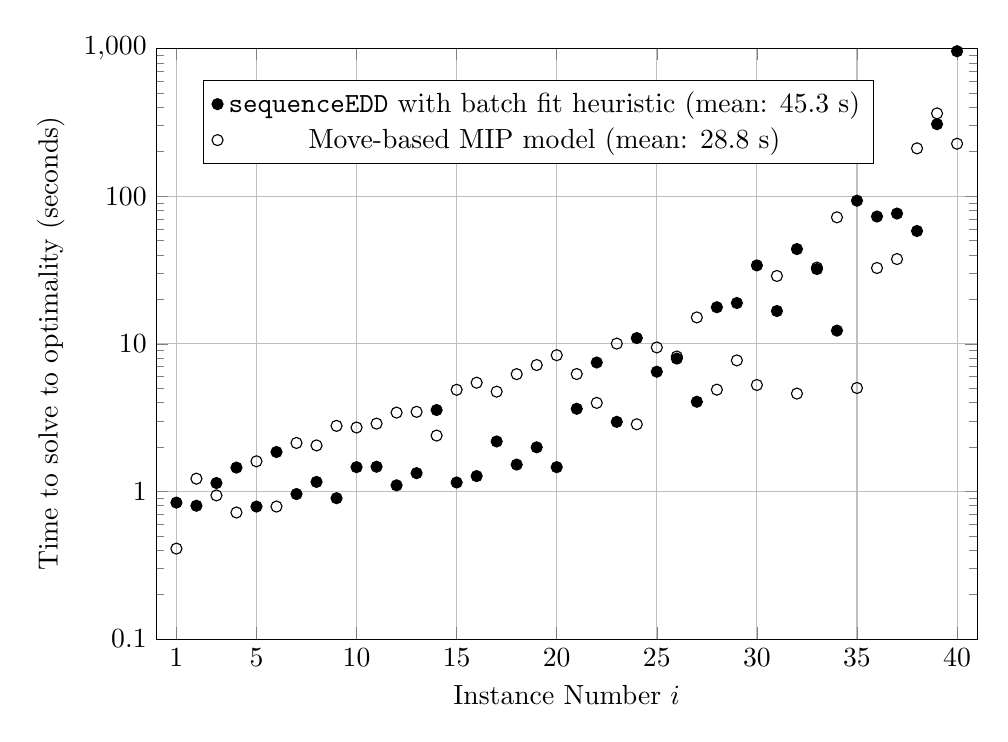
\begin{tikzpicture}

  \begin{semilogyaxis}[width=0.99\textwidth, 
  height=0.749\textwidth,legend pos=north west, xmin=0, xmax=41, ymin=0.1,
  ymax=1000.0, xtick={1,5,10,15,20,25,30,35,40}, y tick label style={
        /pgf/number format/.cd,
            fixed,
            fixed zerofill,
            precision=2,
        /tikz/.cd
    }, log ticks with fixed point, 
    every axis legend/.append style={xshift=8pt, yshift=-5pt}, ylabel=Time to
    solve to optimality (seconds), xlabel=Instance Number $i$,grid]

\addplot[color=black, mark=none,only marks] coordinates {
(1, 0.84)
(2, 0.8)
(3, 1.14)
(4, 1.45)
(5, 0.79)
(6, 1.85)
(7, 0.96)
(8, 1.16)
(9, 0.9)
(10, 1.46)
(11, 1.47)
(12, 1.1)
(13, 1.33)
(14, 3.56)
(15, 1.15)
(16, 1.27)
(17, 2.18)
(18, 1.52)
(19, 1.99)
(20, 1.46)
(21, 3.63)
(22, 7.47)
(23, 2.96)
(24, 10.93)
(25, 6.47)
(26, 7.94)
(27, 4.05)
(28, 17.68)
(29, 18.89)
(30, 33.96)
(31, 16.67)
(32, 43.81)
(33, 32.08)
(34, 12.28)
(35, 93.18)
(36, 72.79)
(37, 76.25)
(38, 58.07)
(39, 307.31)
(40, 958.36)

};
\addlegendentry{\texttt{sequenceEDD} with batch fit heuristic (mean: 45.3 s)}

\addplot[color=black, mark=o,only marks] coordinates {
(1, 0.41)
(2, 1.22)
(3, 0.94)
(4, 0.72)
(5, 1.6)
(6, 0.79)
(7, 2.13)
(8, 2.05)
(9, 2.78)
(10, 2.71)
(11, 2.88)
(12, 3.42)
(13, 3.46)
(14, 2.39)
(15, 4.88)
(16, 5.45)
(17, 4.74)
(18, 6.23)
(19, 7.18)
(20, 8.37)
(21, 6.24)
(22, 3.98)
(23, 10.03)
(24, 2.85)
(25, 9.45)
(26, 8.2)
(27, 15.09)
(28, 4.89)
(29, 7.72)
(30, 5.26)
(31, 28.8)
(32, 4.6)
(33, 32.83)
(34, 71.89)
(35, 5.02)
(36, 32.62)
(37, 37.49)
(38, 210.66)
(39, 363.56)
(40, 226.48)

};
\addlegendentry{Move-based MIP model (mean: 28.8 s)}

  \end{semilogyaxis}
\end{tikzpicture}
   \vspace{0.73em}
\caption{Percentage of problem instances solved in a given
time}\label{fig:malapertresultcomp}
\end{figure}
